\documentclass[12pt]{article}

\usepackage[a4paper,margin=1in]{geometry}
\usepackage{setspace}
\onehalfspacing

\usepackage{amsmath,amssymb,amsthm}
\usepackage{graphicx}
\usepackage{float}
\usepackage{caption}
\usepackage{subcaption}
\usepackage{enumitem}

\title{ECON 5345 Homework 10 Report}
\author{Harlly Zhou}
\date{\today}

\begin{document}

\maketitle

Figure \ref{fig:1} shows the MCMC chain for the parameters.
\begin{figure}[htbp]
    \centering
    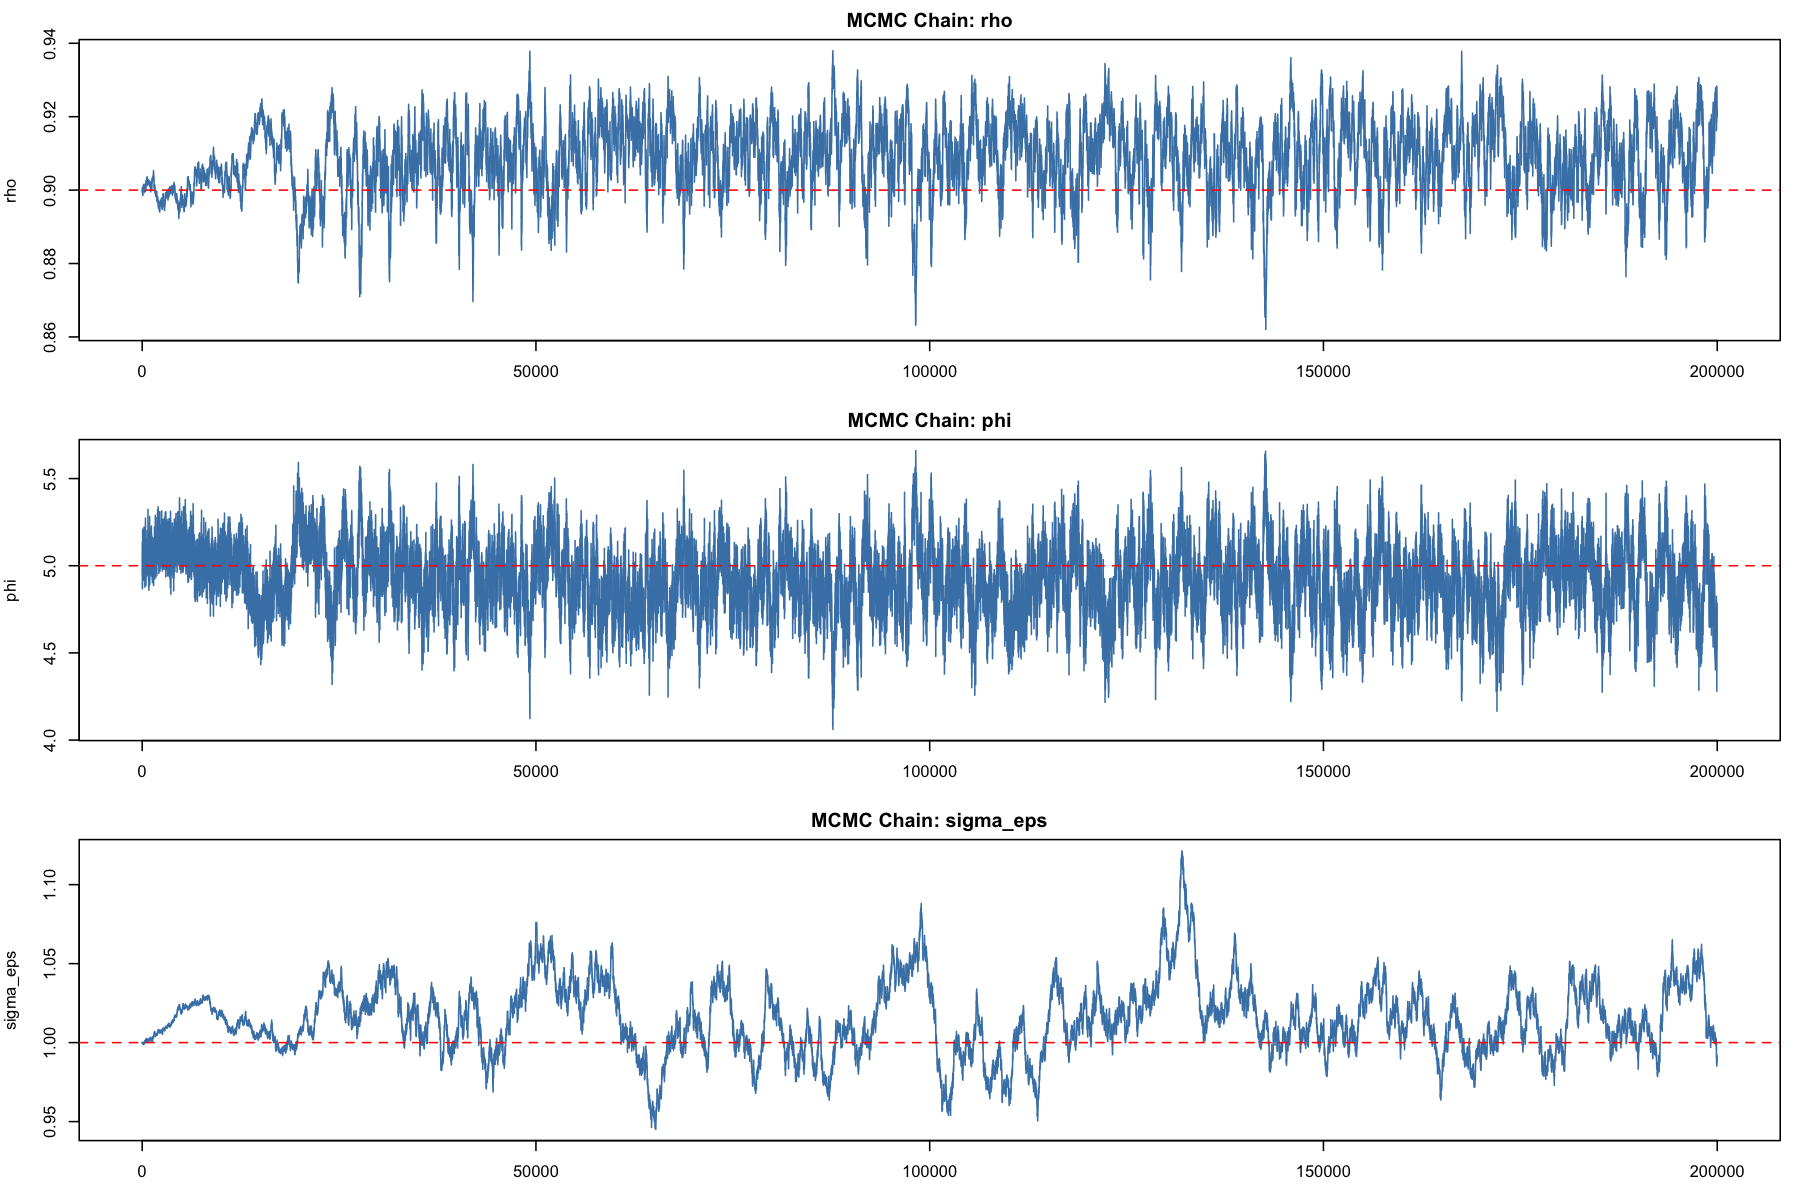
\includegraphics[width=0.6\textwidth]{hw10_output/hw10_chain_plots.png}
    \caption{MCMC chain for the parameters}
    \label{fig:1}
\end{figure}

$\rho$ and $\phi$ are very likely to have converged, while I am not that sure about $\sigma_{\varepsilon}$. It seems that each period is longer for $\sigma_{\varepsilon}$ than for the other two parameters.

Figure \ref{fig:2} shows the path of objective function value.
\begin{figure}[htbp]
    \centering
    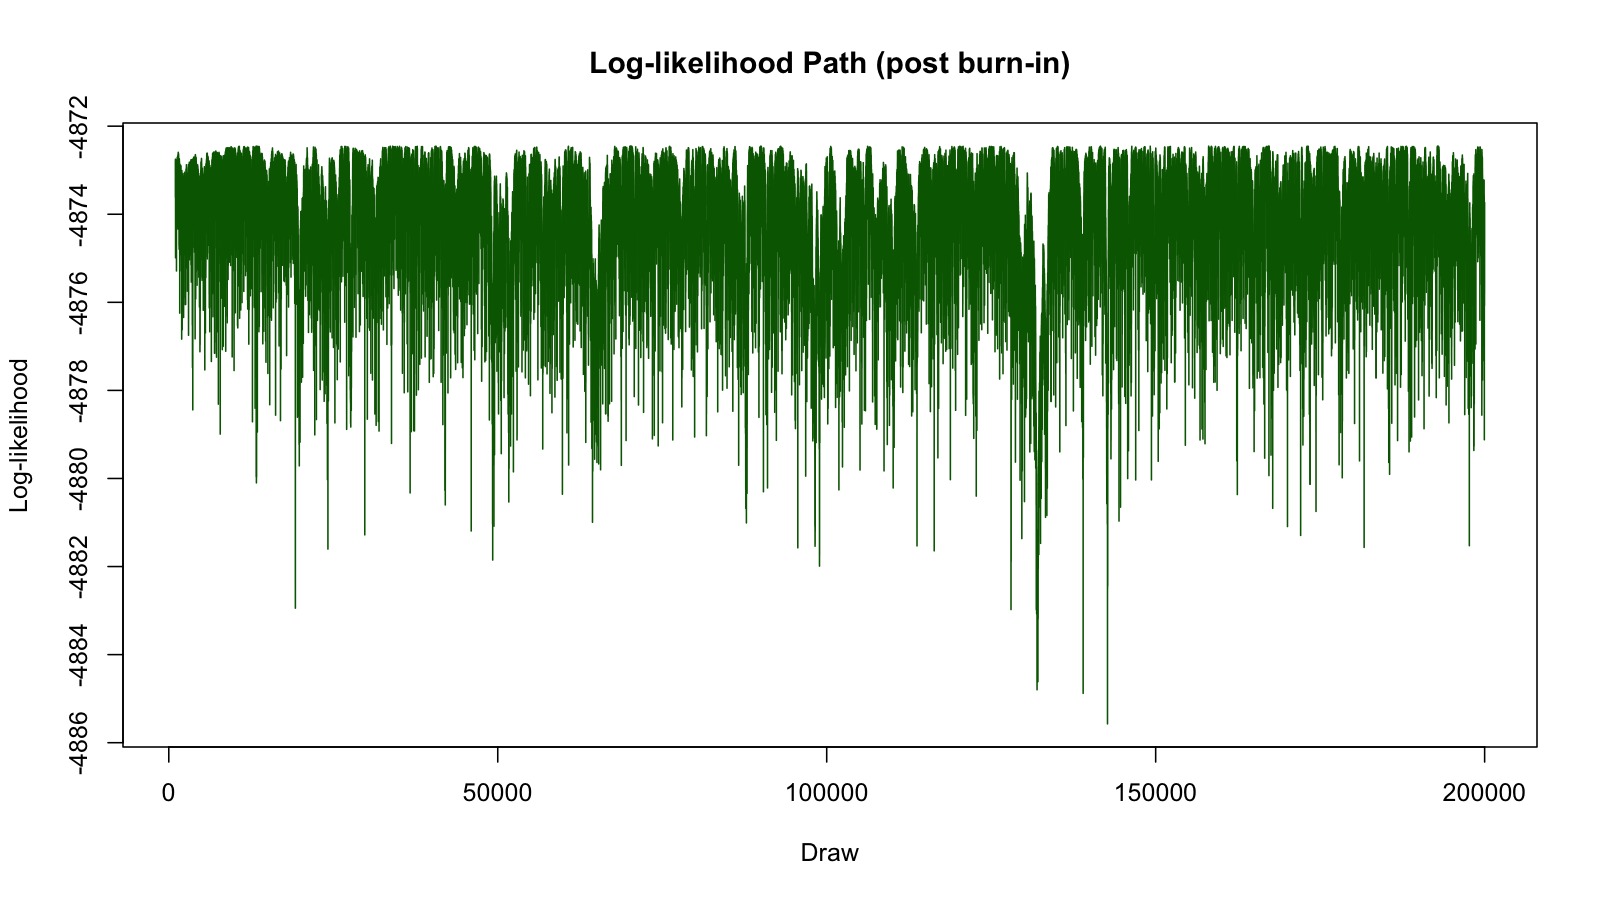
\includegraphics[width=0.6\textwidth]{hw10_output/hw10_objective_path.png}
    \caption{Path of objective function value}
    \label{fig:2}
\end{figure}

It converges to some value around -4874.

Figure \ref{fig:3} shows the scatter plot of the parameters and the objective function value.
\begin{figure}[htbp]
    \centering
    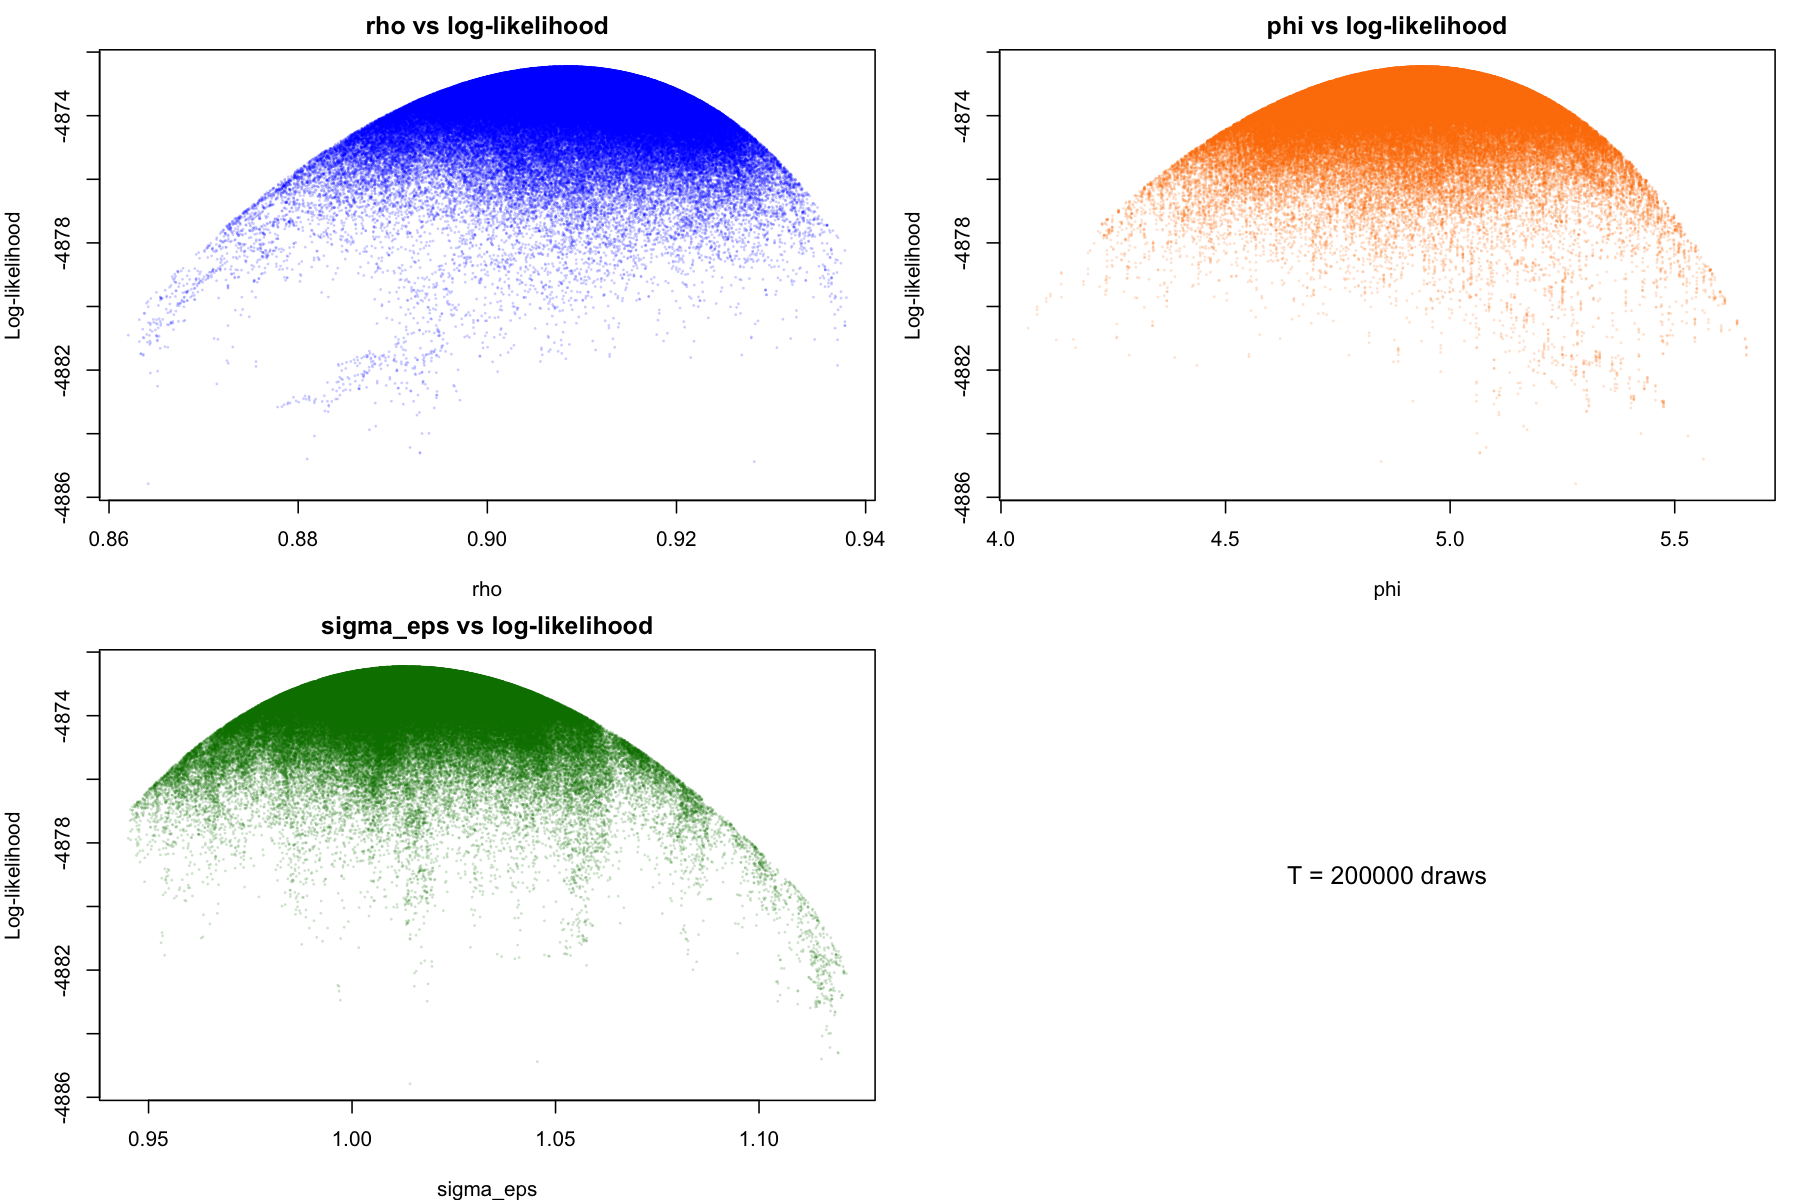
\includegraphics[width=0.6\textwidth]{hw10_output/hw10_scatter_vs_objective.png}
    \caption{Scatter plot of the parameters and the objective function value}
    \label{fig:3}
\end{figure}

The more solid an area is, the more pairs of the parameters and the objective function value are in that area. This means that the values are converging to that area. 


\end{document}
